\section{Tesztelés}

Az alábbi felsorolások a szoftver aktuális állapotának futó verzióján általam
kipróbált műveleteket és azok eredményeit tartalmazzák funkciók szerint
csoportosítva.

 - Sok drón (40 kopter, 0.3s delay)

\subsection{Hőtérképes megjelenítés}

\begin{itemize}

  \item Egy hőtérkép réteg létrehozása után a feliratkozások beállítását
  követően azonnal elkezdenek megjelenni a mérési pontok a téképen.

  \item A színezési függvény, az értékhatárok és a színtartomány bármelyikének
  átállítását követően az "UPDATE PARAMETERS" gomb a jelölők újrarajzolását
  eredményezi a módosított paraméterek tekintetében.

\end{itemize}


\subsection{Térkép állapotainak (pozíció, forgatás, nagyítás) tárolása és betöltése}

\begin{itemize}

  \item Aktuális pozíció eltárolására szolgáló listaelemre kattintva megnyílik
  az adatainak szerkesztésére szolgáló dialógusablak, melyben a bejegyzés neve
  megadható, a mentés véglegesíthető vagy pedig megszakítható. A mentést
  választva a bejegyzés hozzáadódik a lista aljára.

  \item Egy elmentett pozícióhoz tartozó listaelemre kattintva a térkép betölti
  a hozzá tartozó állapotot.

  \item Egy elmentett pozíció listaeleme melletti fogaskerék ikonra kattintva
  megnyílik az annak szerkesztésére szolgáló dialógusablak, melyből
  módosíthatóak a hozzá tartozó paraméterek, a végrehajtott módosítások
  elmenthetők vagy pedig elvethetőek, továbbá a teljes bejegyzés is törölhető.

\end{itemize}


\subsection{Objektumok betöltése GeoJSON formátumból}

\begin{itemize}

  \item Hibás tartalom esetén az "IMPORT GEOJSON" gomb megnyomását követően a
  képernyő alsó szélén felugró üzenet jelzi, hogy helytelen a GeoJSON adat. Az
  üres mező is hibás adatnak számít, hiszen a nulla hosszúságú sztring nem valid
  GeoJSON. (A mező kezdeti értéke "{}".) A bevitt adat ekkor nem kerül
  rögzítésre, így a legultolsó valid tartalom marad kirajzolva a térképre.

  \item Helyes tartalom esetén az import "IMPORT GEOJSON" gombra kattintva az
  adat által leírt objektumok megjelennek a térképen a beállított kitöltési és
  körvonalazási színekkel. Az előzőleg megjelenített objektumok eltűnnek, tehát
  több különálló adat kirajzolásához több GeoJSON réteg létrehozása szükséges.

\end{itemize}


\subsection{Parancsok kiadása drónoknak menüsorról és jobb egérgombra felugró ablakból}

\begin{itemize}

  \item Amennyiben egy drón sincs kijelölve, akkor a jobb klikk menüben és az
  eszköztárban is inaktívak (tehát szürkék és nem kattinthatóak) a gombok.

  \item Legalább egy kijelölt drón esetén a gombok aktívvá válnak.

  \item Egy parancshoz tartozó gombra történő kattintás után a drónok
  végrehajtják a kapott parancsot (a teszt szerver által szimulált drónok csak a
  leszállás és felszállás parancsok végrehajtását támogatják), az eseménynaplóba
  pedig bejegyzés kerül, amikor visszajelzés érkezik a szervertől, hogy
  megérkezett hozzá az utasítás kiadását kezdeményező üzenet.

\end{itemize}


\subsection{Állapotüzenetek (információk, figyelmeztetések, hibák) kijelzésére alkalmas panel}

\begin{itemize}

  \item Új állapotüzenet érkezésekor a táblázat megjeleníti a bejegyzést.

\end{itemize}


\subsection{Drónok színkódolása predikátumok alapján}

\begin{itemize}

  \item Üresen hagyott mező esetén a szín egyik drónra sem érvényesül.

  \item Helyesen kitöltött mező esetén az "APPLY CHANGES" gomb (vagy az Enter
  billentyű) megnyomása után a szín a feltételt teljesítő drónokra érvényesül.

  \item Hibásan kitöltött mező esetén az "APPLY CHANGES" gomb (vagy az Enter
  billentyű) megnyomását követően a hibás mező címkéje és alsó szegélye piros
  színre vált, a hiba szövege bekerül az eseménynaplóba. A bevitt érték nem
  kerül rögzítésre, tehát a szín azokra a drónokra marad érvényes, amelyek a
  mező által előzőleg tartalmazott legutolsó valid predikátumot teljesítik.

\end{itemize}


\subsection{Drónok részletes aktuális állapotát mutató panel}

\begin{itemize}

  \item A táblázat helyesen kijelzi a drónokról jelenleg ismert információkat.

\end{itemize}


\subsection{Kliens állomás pozíciójának megjelenítése a térképen geolokáció alapján}

\begin{itemize}

  \item Ha nem érhető el pozícióra vonatkozó adat (telsztelve asztali
  böngészőben letiltva a geolokációt, illetve mobiltelefonon kikapcsolva a
  GPS-t), akkor a jelölő nem kerül rá a térképre és az eseménynaplóban
  megjelenik egy erre vonatkozó bejegyzés.
  \begin{figure}[H]
    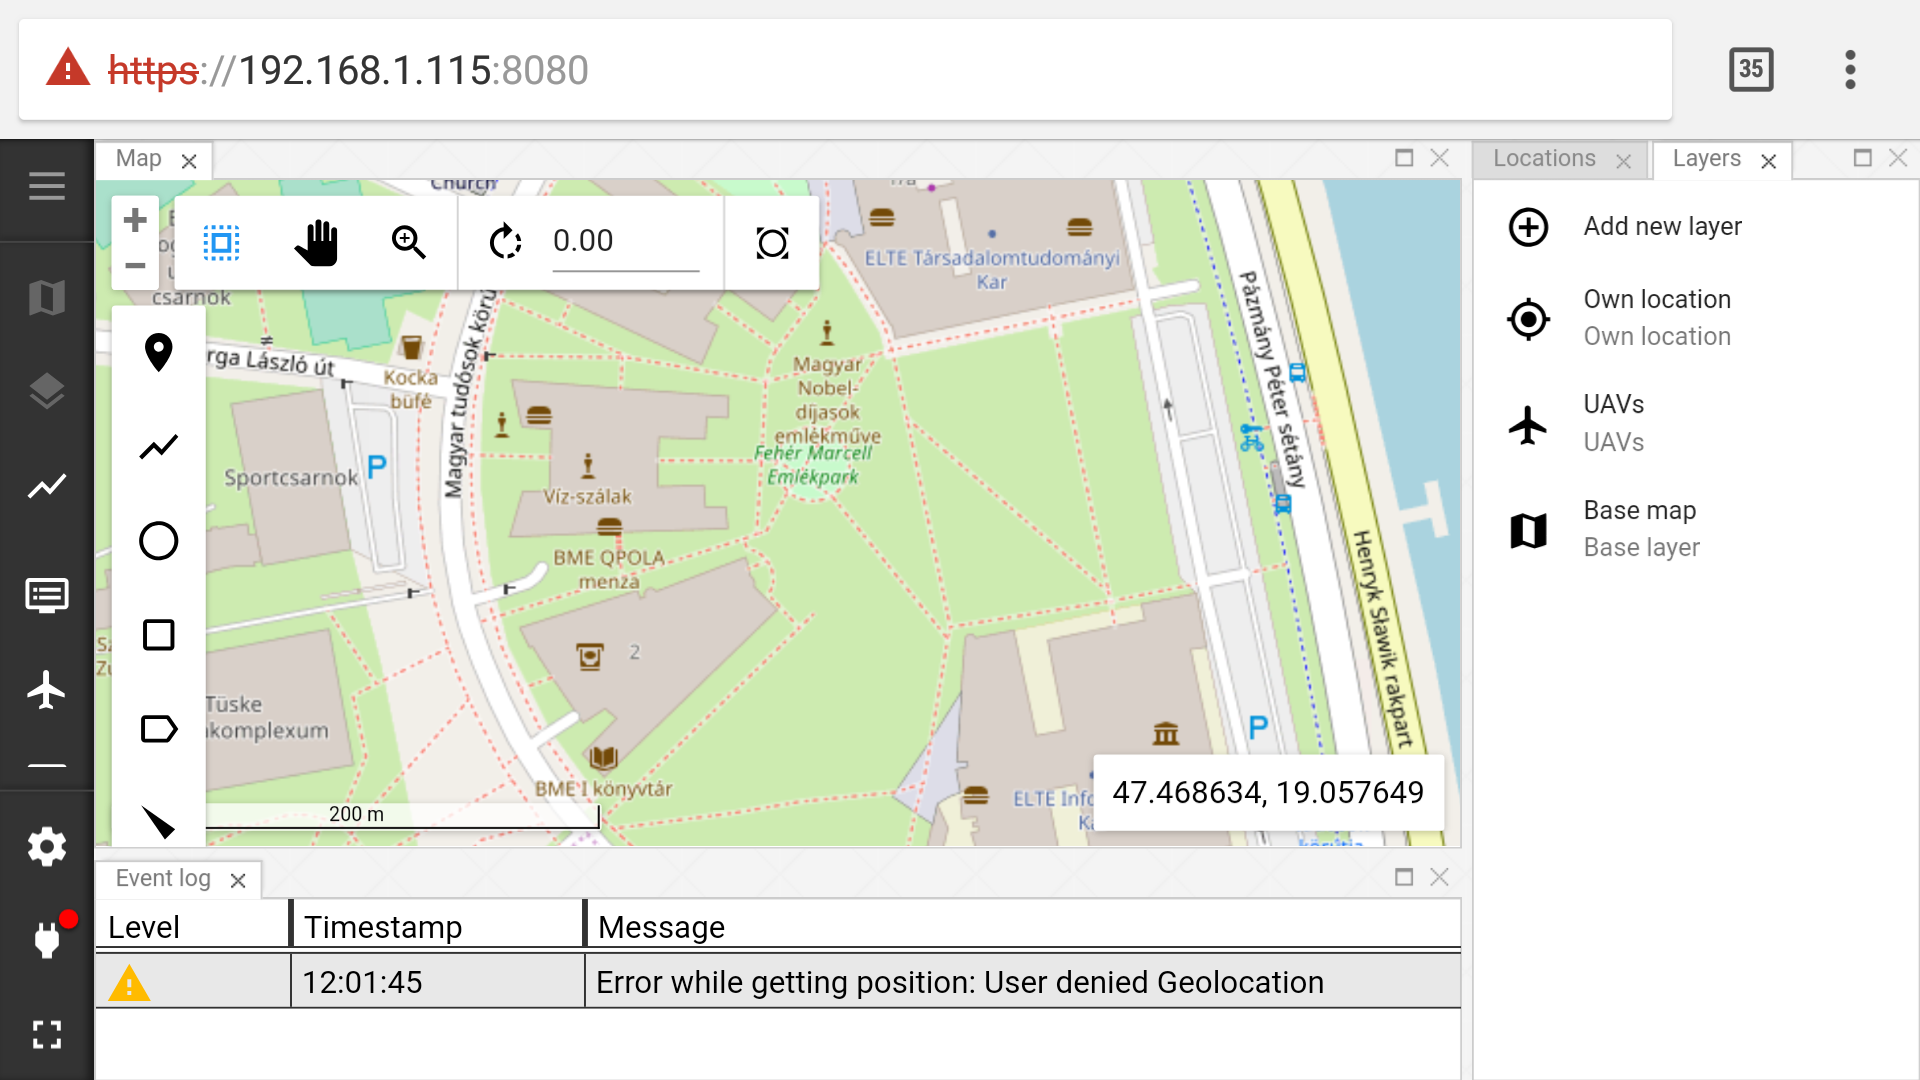
\includegraphics[width=\textwidth]{phone_gps_denied.png}
    \caption{Mobil eszköz kikapcsolt GPS-el}
    \label{fig:phone_gps_denied}
  \end{figure}

  \item Ha elérhető geolokáció szolgáltatás, akkor a jelölő felkerül a térkép
  megfelelő pontjára, valamint a pozíció megváltozásakor frissül és követi az
  elmozdulást.

  \item Ha elérhető mágneses orientációérzékelő is az eszközben, akkor a jelölő
  követi annak elfordulását.
  (Ez a funckió már előzőleg működőképes volt, azonban hoszzú időn át nem került
  sor az ellenőrzésére annak köszönhetően, hogy mágneses érzékelő általában csak
  mobiltelefonokban van. Laptopról legfeljebb csak emulálni lehet, a telefonról
  történő teszteléshez pedig publikus https szerver indítása szükséges, mert a
  geolokációhoz csak titkosított (vagy megbízható, például "localhost")
  kapcsolat esetén biztosítanak hozzáférést a modern böngészők. Ebből adódott,
  hogy csak most, miután tesztelés közben nem működött, derült fény arra, hogy
  az eredeti megvalósításához használt, OpenLayers könyvtárból származó
  DeviceOrientation osztály a legutóbbi verzióban már elavultnak lett
  nyilvánítva és a tapasztalat alapján nem is funckcionál rendesen. Áttérve a
  közvetlenül a böngésző által rendelkezésre bocsátott "deviceorientation"
  esemény figyelésére újra működésbe lépett a funkció, mint az a képen
  (\ref{fig:phone_compass}. ábra) is látható.)

  \begin{figure}[H]
    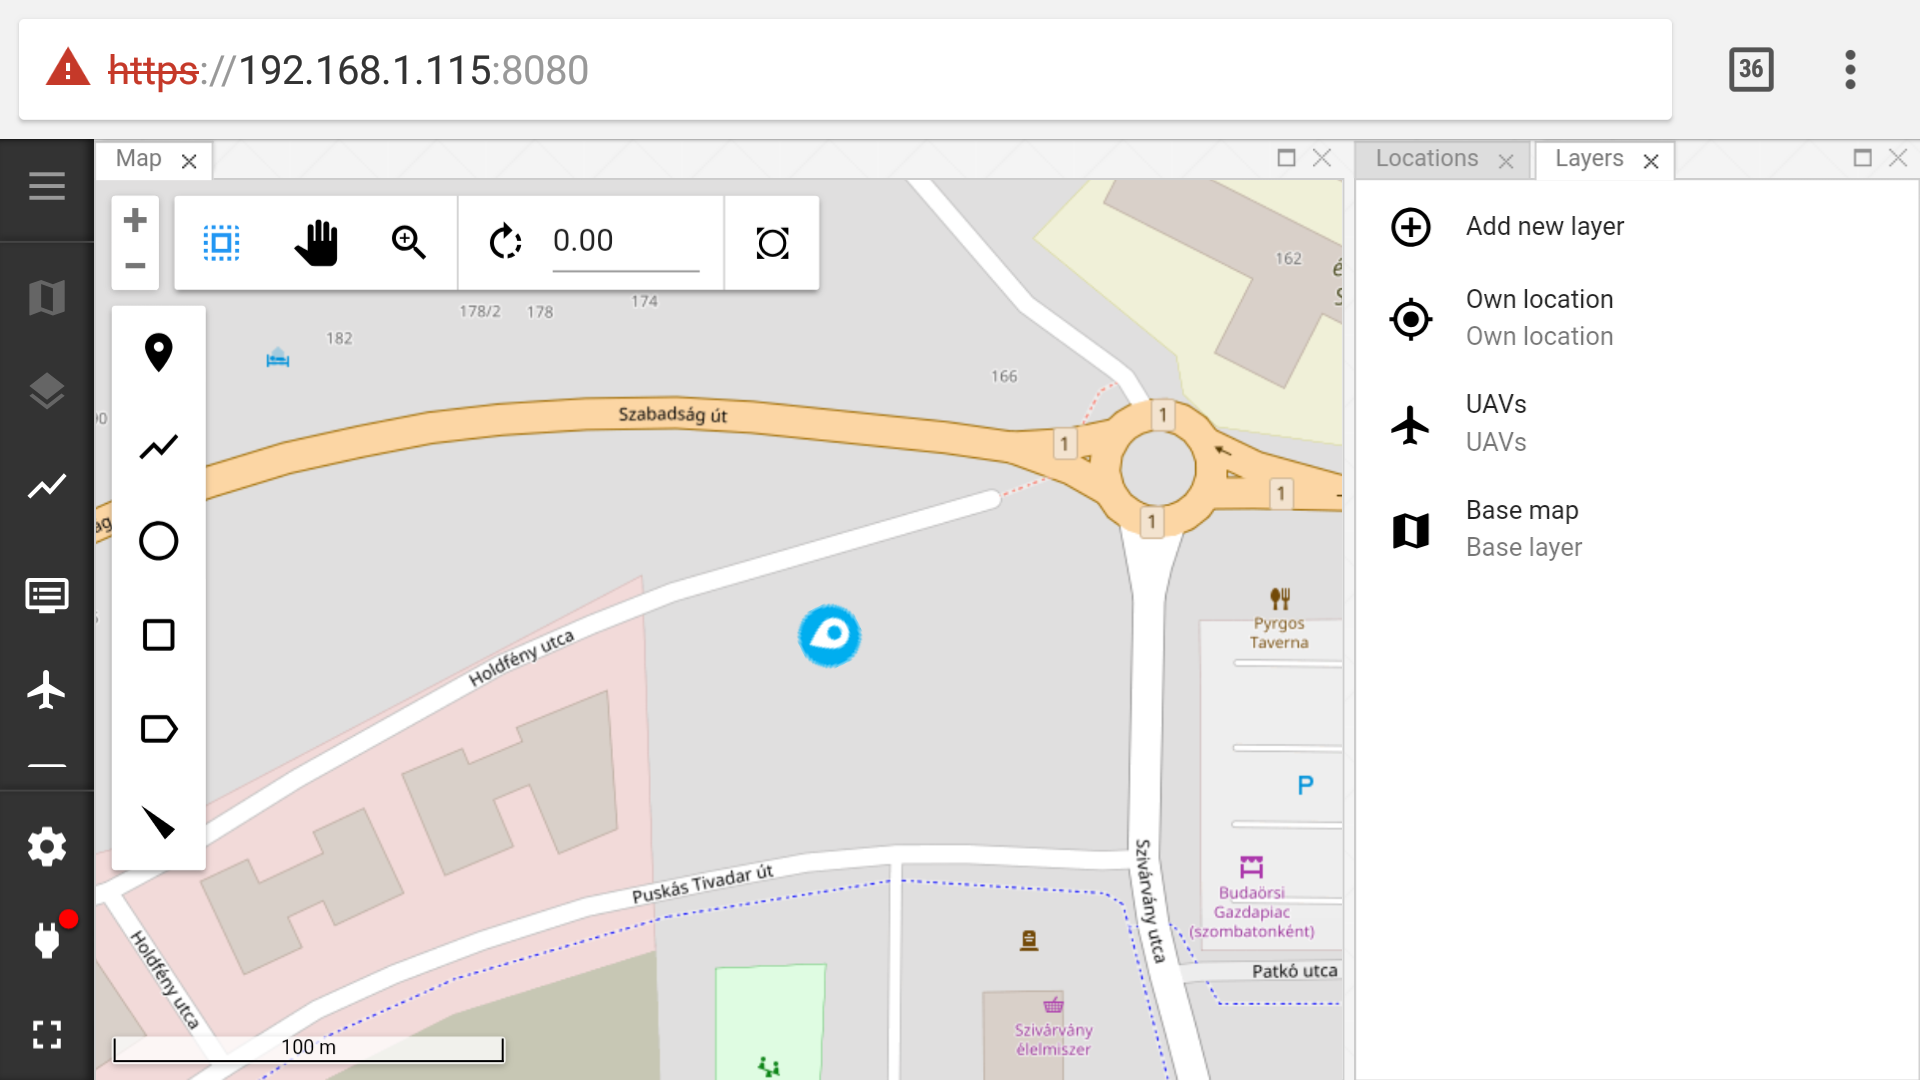
\includegraphics[width=\textwidth]{phone_compass.png}
    \caption{Iránytű alapján elforduló jelölő mobil eszközön}
    \label{fig:phone_compass}
  \end{figure}

\end{itemize}


\subsection{Billentyűkombinációkkal történő vezérlés}

\begin{itemize}

  \item Minden billentyűkombináció megfelelően működik.

\end{itemize}


\subsection{Nagy mennyiségű drón kezelése}

Hatékonyság szempontjából a felület tesztelésre került különböző számú szimulált
drónnal változatos üzenetsűrűségekkel. A tapasztalat az, hogy 40 kopter esetén
nagyjából (drónonként) 0.3 másodpercenként érkező üzenetek esetén éri el az
alkalmazás aktív használat közben egy 2.5GHz-es órajelen üzemelő processzormag
kapacitásának határait. Ekkor a felület még használható marad, de már elkezdenek
szaggatni az animációk. Ezek alapján a szoftver bár képes a kitűzött cél
ellátására, azért a felhasználói élmény javításának érdekében még további
optimalizációra szorul a későbbiekben.
